\subsection{齐性空间}

设 G 是一个拓扑群，H 是 G 的一个子群。H 依照外法则 \((t, x) \to xt\) 在 G 的右边连续作用，且点 \(x \in G\) 的轨道是左陪集 xH。因此诸轨道组成的集就是我们在代数中所谓的齐性空间 G/H。每当我们把 G/H 作为拓扑空间谈论时，除相反的情况有明确说明外，所指的总是 G 的轨道空间（关于 H 的）；即 G 关于等价关系 \(x^{-1}y \in H\) 的商空间。按照一般定义，我们说这个空间的拓扑是 G 的拓扑经 H 的商。

命题 12 群 G 在每个齐性空间 G/H 上连续作用。

由于等价关系 \(x^{-1}y \in H\) 是开的（第 4 目引理 2），这是第 4 目命题 11 的一个特殊情形。

命题 13 设 G 是一个拓扑群，H 是 G 的一个子群。则齐性空间 G/H 是 Hausdorff 的，当且仅当 H 在 G 中是闭的。

H 是关系 \(x^{-1}y \in H\) 的一个等价类，因此若 G/H 是 Hausdorff 的，则 H 在 G 中是闭的。反之，若 H 是闭的，则这个关系的图在 \(G \times G\) 中是闭的，因为它是 H 在连续映射 \((x, y) \to x^{-1}y\) 下的原像。由于关系 \(x^{-1}y \in H\) 是开的，由第一章 § 8 第 3 目命题 8 可知 G/H 是 Hausdorff 的。

命题 14 设 G 是一个拓扑群，H 是 G 的一个子群。则齐性空间 G/H 是离散的，当且仅当 H 在 G 中是开的。

因为在典范映射下 G/H 的诸点在 G 中的原像是诸陪集 xH（x ∈ G）；而这些集合在 G 中是开的，当且仅当 H 在 G 中是开的。

设 X 是一个拓扑空间，拓扑群 G 连续且可迁地作用在它上面；这时 X（在代数意义上）是 G 的一个齐性空间。设 \(x\) 是 \(X\) 的一点，\(H_x\) 是它的稳定子群。连续满射 \(s \to s.x\)（\(G\) 到 \(X\) 上的）典范地分解为

\[
\mathbf {G} \xrightarrow {f _ {x}} \mathbf {G} / \mathbf {H} _ {x} \xrightarrow {g _ {x}} \mathbf {X}
\]

\pandocbounded{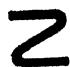
\includegraphics[keepaspectratio]{images/part002_c9cfa224.jpg}}

其中 \(f_x\) 是 \(G\) 到齐性空间 \(G/H_x\) 上的典范映射，\(g_x\) 是双射 \(s.H_x \to s.x\)（\(G/H_x\) 到 \(X\) 上的）；此外（第一章 § 3 第 4 目命题 6），\(g_x\) 是连续映射。但 \(g_x\) 未必是 \(G/H_x\) 到 \(X\) 上的一个同胚（习题 29）。若 \(g_x\) 对每个 \(x \in X\) 都是同胚，则称 \(X\)（拓扑群 \(G\) 的）为拓扑齐性空间；为此的充要条件是：对每个 \(x \in E\)，映射 \(s \to s.x\)（\(G\) 到 \(X\) 中的）是开的。

命题 15 设 X 是一个拓扑空间，拓扑群 G 连续且可迁地作用在它上面。为使 X 是（关于 G 的）拓扑齐性空间，只需对某一点 \(x_{0} \in X\)，映射 \(s \to s \cdot x_{0}\) 把 e 在 G 中的每个邻域变换为 \(x_{0}\) 在 X 中的一个邻域。

每个 \(x \in X\) 都可写作 \(x = t.x_0\)（对某个 \(t \in G\)）。若 \(V\) 是 \(e\) 的一个邻域，则 \(V.x = (Vt).x_0\) 是 \(x\) 的一个邻域，因为可以写 \((Vt).x_0 = t((t^{-1}Vt).x_0)\)，而断言由下列事实得出：\(t^{-1}Vt\) 是 \(e\) 在 \(G\) 中的一个邻域，且 \(y \to t.y\) 是 \(X\) 到其自身的一个同胚（第 4 目引理 1）。由此可得，若 \(U\) 是 \(G\) 的任一开子集且 \(x\) 是 \(X\) 的任一点，则 \(U.x\) 在 \(X\) 中是开的；因为若 \(t \in U\)，则 \(t^{-1}U\) 是 \(e\) 的一个邻域，因而 \((t^{-1}U).x\) 是 \(x\) 的一个邻域，且 \(t.((t^{-1}U).x) = U.x\) 是 \(t.x\) 的一个邻域。于是 \(U.x\) 在 \(X\) 中是开的，从而映射 \(s \to s.x\)（\(G\) 到 \(X\) 中的）是开的。证毕。

